%%%%%%%%%%%%%%%%%%%%%%%%%%%%%%%%%%%%%%%%%
% Beamer Presentation
% LaTeX Template
% Version 1.0 (10/11/12)
%
% This template has been downloaded from:
% http://www.LaTeXTemplates.com
%
% License:
% CC BY-NC-SA 3.0 (http://creativecommons.org/licenses/by-nc-sa/3.0/)
%
%%%%%%%%%%%%%%%%%%%%%%%%%%%%%%%%%%%%%%%%%

%----------------------------------------------------------------------------------------
%	PACKAGES AND THEMES
%----------------------------------------------------------------------------------------

\documentclass[aspectratio=149]{beamer}
\usefonttheme[onlymath]{serif}


\mode<presentation> {

% The Beamer class comes with a number of default slide themes
% which change the colors and layouts of slides. Below this is a list
% of all the themes, uncomment each in turn to see what they look like.

\usetheme{default}
%\usetheme{AnnArbor}
%\usetheme{Antibes}
%\usetheme{Bergen}
%\usetheme{Berkeley}
%\usetheme{Berlin}
%\usetheme{Boadilla}
%\usetheme{CambridgeUS}
%\usetheme{Copenhagen}
%\usetheme{Darmstadt}
%\usetheme{Dresden}
%\usetheme{Frankfurt}
%\usetheme{Goettingen}
%\usetheme{Hannover}
%\usetheme{Ilmenau}
%\usetheme{JuanLesPins}
%\usetheme{Luebeck}
%\usetheme{Malmoe}
%\usetheme{Marburg}
%\usetheme{Montpellier}
%\usetheme{PaloAlto}
%\usetheme{Pittsburgh}
%\usetheme{Rochester}
%\usetheme{Singapore}
%\usetheme{Szeged}
%\usetheme{Warsaw}

% As well as themes, the Beamer class has a number of color themes
% for any slide theme. Uncomment each of these in turn to see how it
% changes the colors of your current slide theme.

%\usecolortheme{albatross}
\usecolortheme{beaver}
%\usecolortheme{beetle}
%\usecolortheme{crane}
%\usecolortheme{dolphin}
%\usecolortheme{dove}
%\usecolortheme{fly}
%\usecolortheme{lily}
%\usecolortheme{orchid}
%\usecolortheme{rose}
%\usecolortheme{seagull}
%\usecolortheme{seahorse}
%\usecolortheme{whale}
%\usecolortheme{wolverine}

%\setbeamertemplate{footline} % To remove the footer line in all slides uncomment this line
%\setbeamertemplate{footline}[page number] % To replace the footer line in all slides with a simple slide count uncomment this line

%\setbeamertemplate{navigation symbols}{} % To remove the navigation symbols from the bottom of all slides uncomment this line
}

\usepackage{graphicx} % Allows including images
\usepackage{booktabs} % Allows the use of \toprule, \midrule and \bottomrule in tables
\usepackage{verbatim}

\usepackage{mathtools} 
\usepackage{amssymb}
\usepackage{mathrsfs}
\usepackage{amsmath}

\usepackage{ragged2e}
\usepackage{etoolbox}
\usepackage{lipsum}

\usepackage{siunitx,booktabs}
\usepackage{pifont}



\setbeamertemplate{enumerate items}[circle]
\usepackage{tikz}

\newcommand\mynum[1]{
  \usebeamercolor{enumerate item}
  \tikzset{beameritem/.style={circle,inner sep=0,minimum size=2ex,text=enumerate item.bg,fill=enumerate item.fg,font=\footnotesize}}%
  \tikz[baseline=(n.base)]\node(n)[beameritem]{#1};
}

\newcommand\mynumm[1]{
  \usebeamercolor{enumerate item}
  \tikzset{beameritem/.style={rectangle,inner sep=0,minimum size=2ex,text=enumerate item.bg,fill=enumerate item.fg,font=\footnotesize}}%
  \tikz[baseline=(n.base)]\node(n)[beameritem]{#1};
}

\def\Put(#1,#2)#3{\leavevmode\makebox(0,0){\put(#1,#2){#3}}}

\setbeamertemplate{footline}[frame number]

%----------------------------------------------------------------------------------------
%	TITLE PAGE
%----------------------------------------------------------------------------------------

\title{ Subsidized Housing in the Developping World: Evidence from South Africa } % The short title appears at the bottom of every slide, the full title is only on the title page

\author{Stefano Polloni \\
joint with Ben Bradlow and Will Violette} 

 % Your institution as it will appear on the bottom of every slide, may be shorthand to save space

\date{September 2017} %\today} % Date, can be changed to a custom date

\begin{document}

\beamertemplatenavigationsymbolsempty

\begin{frame}
\titlepage % Print the title page as the first slide
\end{frame}

%\begin{frame}
%\frametitle{Overview} % Table of contents slide, comment this block out to remove it
%\tableofcontents % Throughout your presentation, if you choose to use \section{} and \subsection{} commands, these will automatically be printed on this slide as an overview of your presentation
%\end{frame}

%----------------------------------------------------------------------------------------
%	PRESENTATION SLIDES
%----------------------------------------------------------------------------------------
\section{Introduction}
%------------------------------------------------

\begin{frame}
\frametitle{Motivation}

\begin{itemize}
\item Rapid Urbanization of the developping world during the past two decades. 
\vspace{1mm}
\vspace{1mm}
\item Significant portion of new city-dwellers live in slums.
\vspace{1mm}
\begin{itemize}
\item Africa's estimated slum population doubled in 1995-2015.
\end{itemize}
\vspace{1mm}
\item Disagreement on whether slum-dwellers are in a transitory phase (Glaeser, 2011) or stuck in proverty traps (Marx, 2013). 
\vspace{1mm}
\item Regardless, slum living conditions remain a concern:
\vspace{1mm}
\begin{itemize}
\item inadequate living space
\item poor sanitation and water access
\item high crime levels
\item low public goods provision



\end{itemize}
\vspace{1mm}
\end{itemize}

\end{frame}

%------------------------------------------------

\begin{frame}
\frametitle{Motivation}

Standard policy portfolio to address these issues:

\vspace{2mm}

\begin{enumerate}
\item Changing property rights and land regulations
  \begin{itemize}
    \item land titling (Galiani \& Shargrodoksy 2010, Field 2007) 
    \item reducing minimum lot size (Lall et al. 2007)
  \end{itemize}
\vspace{1mm}
\item On-site slum upgrading/servicing (Galiani et al. 2017, Field and Kremer 2008)
\vspace{1mm}
\item Subsidized formal housing (Picarelli 2017, Barnhardt et al 2015)
\end{enumerate}
\vspace{1mm}
Due to data constraints and lack of experimental variation, evidence for each three remains scarce, with no answer on the best policy mix. 

\end{frame}

%------------------------------------------------

\begin{frame}
\frametitle{This Paper:}

\begin{itemize}
\item Focus on {\!\!\!\mynum{3}}, the provision of subsidized  housing.
\item Learn from the South African experience with post-apartheid Reconstruction and Development Programme (RDP):
\begin{itemize}
    \item Since 1994, delivery of $\sim$\! 3 million freestanding houses across the country for households with income $<$ \$R3500 (\$260) per month.
  \end{itemize}
\vspace{2mm}
\item Existing literature in development economics treats subsidized housing as relocation programs (e.g. MTO), focusing mainly on outcomes of relocated households.

\item Subsidized housing is also a place-based policy that affects the surrounding neighborhoods. (Diamond \& McQuade 2016)

\item These external effects have been studied in the developed world (Diamond \& McQuade 2016, Baum-Snow \& Marion 2009, Schwartz et al. 2006), but not in a slum mitigation context. 

\end{itemize}


\end{frame}

%------------------------------------------------

\begin{frame}
\frametitle{Research Questions}
  \begin{enumerate}
    \setbeamertemplate{enumerate items}[square]
    \item What is the value of subsidized housing to both {\bf recipients} and {\bf surrounding residents}? How does this depend on the location and density of delivered units?
    \item How does the provision of public housing impact the growth of surrounding informal housing?
      \begin{itemize}
    \item many developments built near existing informal settlements.
    \item informal backyard shacks are common occurrence.
  \end{itemize}
  \end{enumerate}
  \vspace{1mm}
\begin{enumerate}
  \setbeamertemplate{enumerate items}[square]
  \setcounter{enumi}{2}
  \item Given {\!\!\!\mynumm{1}}, {\!\!\!\mynumm{2}}, and the costs of construction/land, is this policy successful? 

\vspace{2mm}

  Are there potential welfare improvements in changing how and where housing units are delivered?
\end{enumerate}


\end{frame}


%------------------------------------------------

\begin{frame}
\frametitle{RDP housing in a nutshell }
  \begin{itemize}
    \item The RDP is a policy framework implemented in 1994 to address several socioeconomic issues under apartheid rule.
    \item Includes a large housing subsidy scheme, which provides eligible households the opportunity of owning their first house.
    \item Eligibility is based on citizenship, marital status and income.
    \item Program recipients receive a one-off capital subsidy (the house) at very low or no cost.
    \item Large excess demand; allocation process loosely regulated by various priority systems and wait lists, with many noted cases of corruption.
    \item Supply is planned by municipal and provincial housing agencies, construction is outsourced to private developers, with constraints on costs per unit, services access, and rooms/lot sizes.
  \end{itemize}



\end{frame}


%------------------------------------------------

\begin{frame}
\frametitle{RDP housing as a relocation program }
Previous work has examined RDP housing as a relocation program, tracking households that move from slums into RDP housing. Results are inconsistent.

\vspace{.5em}

Picarelli, 2017:
  \begin{itemize}
    \item Panel Survey 2008-2012, 723 household living in 6 largest metros
    \item Fuzzy RD using \$R3500 threshold for eligibility   
    \item RDP recipient households, on average, are displaced further away from the CDB, and reduce their total labor supply upon receiving their house.
  \end{itemize}

  \vspace{.5em}

Franklin, 2015:
  \begin{itemize}
    \item Panel Survey 2002-2009, 1097 households in Cape Town area 
    \item RDP recipient households report increased earnings, driven by higher female employment rate.
  \end{itemize}




\end{frame}


%------------------------------------------------


\begin{frame}
\frametitle{RDP as a place-based policy}
  \begin{itemize}
    \item RDP houses are usually built as part of extensive residential developments, with considerable heterogeneity in location and density.
    \vspace{2mm}
    \item Their effect may extend well beyond the program recipients, affecting location decisions of other households and the construction decisions of private developers. 
    \vspace{2mm}
    \item Quantifying these effects is important for comprehensive policy evaluation.
  \end{itemize}

\end{frame}


%------------------------------------------------

\begin{frame}
\frametitle{RDP as a place-based policy}
\begin{center}
\begin{figure}
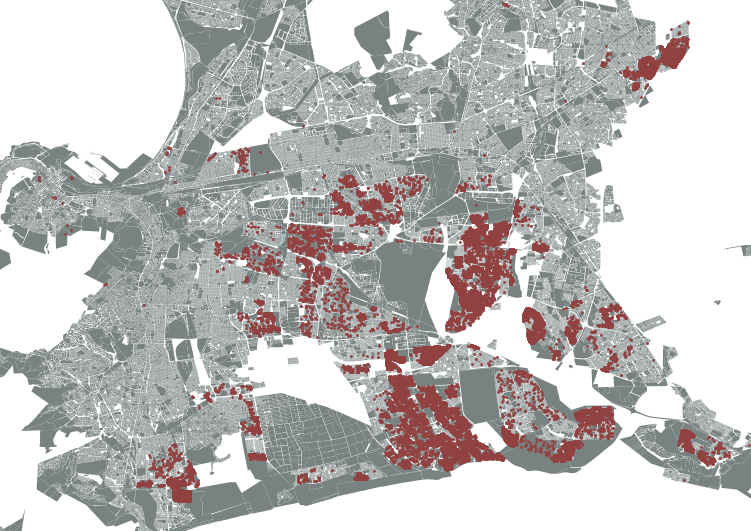
\includegraphics[scale=0.33]{map.png}
\vspace{-3mm}
\caption{RDP properties (in red) surrounding Cape Town}
\end{figure}
\end{center}

\end{frame}


%------------------------------------------------

\begin{frame}
\frametitle{Data Sources}
\vspace{-1em}
{\bf Three main data sources: }

\vspace{1em}

1. Deeds data:
\vspace{2mm}
  \begin{itemize}
    \item Universe of housing transactions recorded during 2003-2011 in all affordable areas\footnote{defined as census enumeration areas with mean house price value less than R500,000 in 2010.} across the country. ($\sim$\! 1.2M transactions)
    \vspace{2mm}
    \item Exact geographic location of traded property, but limited information on characteristics other than price and lot size.
    \vspace{2mm}
    \item RDP transactions noisily identifiable by filtering on Seller Name, price and lot size ($\sim$\! 400K transactions)
\end{itemize}
\end{frame}

\begin{frame}
\frametitle{Data Sources}
2. Buildings inventory data:
\vspace{2mm}
  \begin{itemize}
    \item 2 waves - 2001 and 2012 - of exhaustive building census based on satellite imagery, covering the entire province of Gauteng (contains Johannesburg and Pretoria).
    \vspace{2mm}
    \item building stock differentiable by various categories: residential, commercial, industrial, etc.
    \vspace{2mm}
    \item within residential, ability to differentiate formal from informal housing, including backyard shacks.
    \vspace{2mm}
    \item Hopefully access to National Coverage and more waves very soon...
\end{itemize}
\end{frame}

\begin{frame}
\frametitle{Data Sources}
3. Census data:
\vspace{2mm}
  \begin{itemize}
    \item Full national coverage of the 2001 and 2011 census, at the small area level ($\,\,\sim$ 170 households per small area)
    \vspace{2mm}
    \item  Basic information on demographics, employment, income, education and dwelling characteristics.

\end{itemize}
\end{frame}


%------------------------------------------------

\begin{frame}
\frametitle{Goals with this data}
\begin{enumerate}
\item Estimate impact of RDP construction on surrounding property values.
\vspace{-4mm}
\begin{itemize}
  \item Assess value to neighboring residents in formal housing sector.
\end{itemize}
\vspace{1mm}
\item Estimate the response of informal housing to RDP construction.
\begin{itemize}
  \item Asses value to neighboring residents in informal housing sector.
\end{itemize}
\vspace{1mm}
\item Examine RDP resale transactions to infer value to program recipients.
\vspace{1mm}
\vspace{1mm}
  \item Develop a theoretical framework to map the obtained reduced-from estimates into welfare effects.
  \begin{itemize}
  \item draw from the model in Diamond \& McQuade (2016), or something along the lines of Busso, Gregory and Kline (2013)
\end{itemize}
\end{enumerate}
\end{frame}

%------------------------------------------------

\begin{frame}
\frametitle{Local RDP impact on housing prices}

RDP projects are often built as small neighborhoods on formely empty land plots, or former informal settlements. 

\vspace{1em}


A first-pass DD aproach:
\begin{itemize}
  \item Identify areas where many clustered RDP houses were sold at similar dates.
  \item Examine house prices in adjacent areas, before and after construction, near and far from RDP project.
  \item Rely on spatial proximity for identification. 

\end{itemize}

\end{frame}

%------------------------------------------------

\begin{frame}
\frametitle{Local RDP impact on housing prices}

\begin{itemize}
  \item Issue: the parent project of each RDP unit is not observed in the transaction data, but only geographic coordinates and date when first allocated. 

  \item Solution (?): Use spatial clustering methods to group RDP transactions into projects. 
\end{itemize}


\end{frame}

%------------------------------------------------

\begin{frame}
\frametitle{Local RDP impact on housing prices}

\begin{center}
\begin{figure}
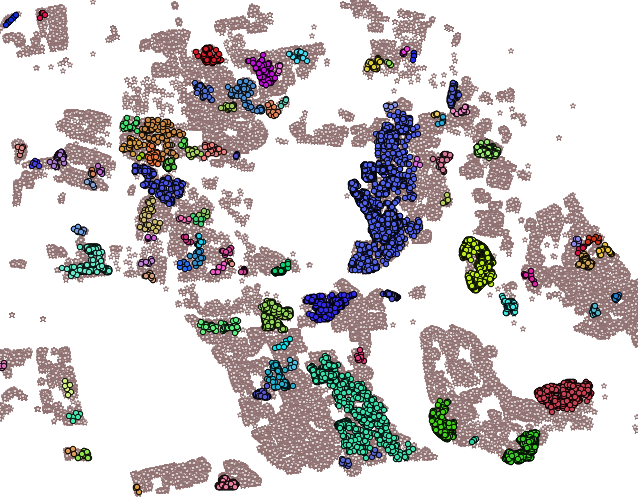
\includegraphics[scale=0.39]{hdbscan.png}
\vspace{-3mm}
\caption{DBScan clustering algorithm}
\end{figure}
\end{center}


\end{frame}

%------------------------------------------------

\begin{frame}
\frametitle{Local RDP impact on housing prices}

Strategy:
\begin{itemize}
\item run DBScan using gps location of RDP transactions.
\item verify that transactions within each identified group occurs closely around the same year. 
\item examine price of non-RDP transactions occuring within a fixed distance of the projects, before and after the mode transaction year.
\end{itemize}


\end{frame}

%------------------------------------------------

\begin{frame}
\frametitle{Local RDP impact on housing prices}
Raw Means:
\begin{center}
\begin{figure}
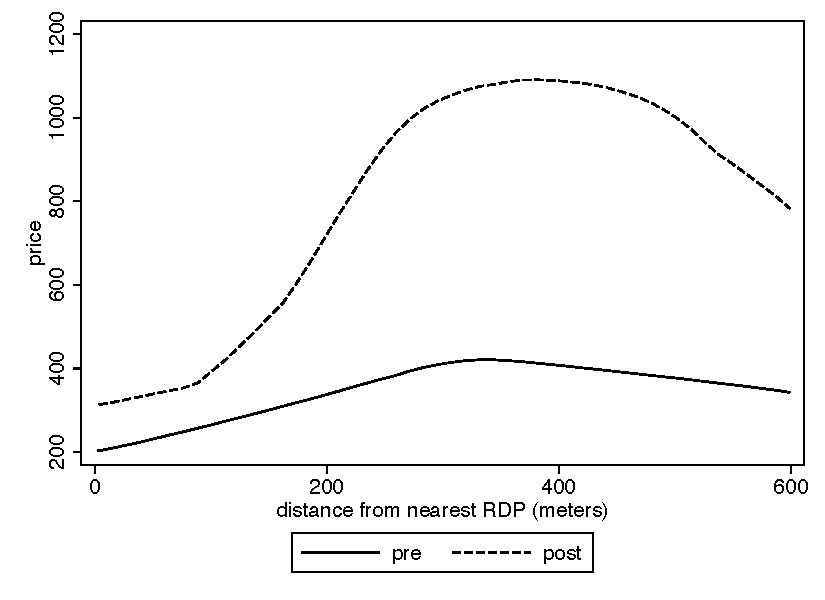
\includegraphics[scale=0.7]{raw_plot2.pdf}
\end{figure}
\end{center}
\end{frame}

%------------------------------------------------

\begin{frame}
\frametitle{Local RDP impact on housing prices}
Net of Province-by-Year-by-Month FE and Project FE:
\begin{center}
\begin{figure}
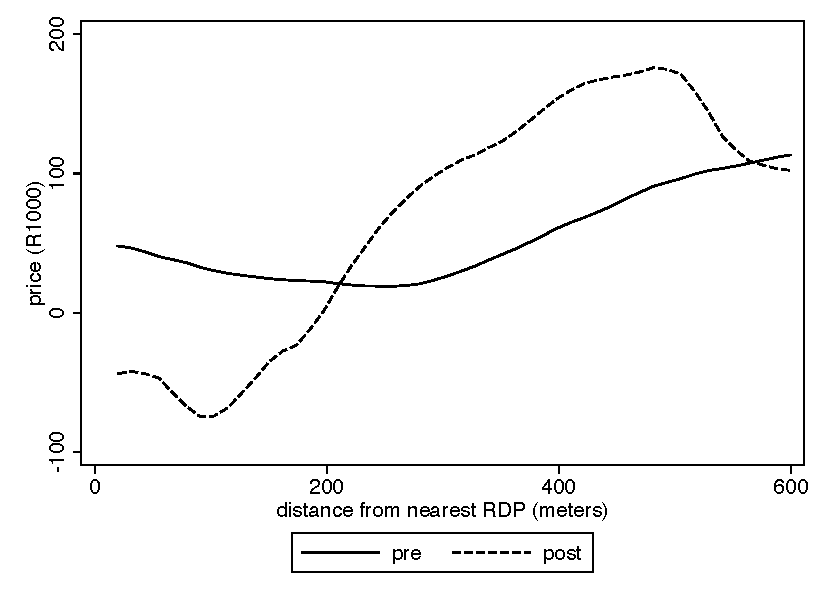
\includegraphics[scale=0.7]{reg_plot2.pdf}
\end{figure}
\end{center}
\end{frame}

%------------------------------------------------


\begin{comment}

\begin{frame}
\frametitle{Goals and Next Steps:}
\vspace{2mm}
\begin{enumerate}
    \setcounter{enumi}{2}
\item Provided I reasonably achieve {\!\!\mynum{1}} and {\!\!\mynum{2}}, develop a theoretical framework to map the obtained reduced-from estimates into welfare effects, answer research question {\!\!\mynumm{3}}.
\begin{itemize}
  \item draw from Diamond 
\end{itemize}
\end{enumerate}
\end{frame}



%------------------------------------------------

\begin{frame}
\frametitle{Data}



\end{frame}

%------------------------------------------------

\begin{frame}
\frametitle{Data}

{\bf Other Data Sources:}

\begin{itemize}
\item Automobile speeds and daily volumes at various location-years around Portland.
\item Geographical Boundaries of 128 Neighborhoods containing houses in dataset.
\item Street grid with detailed hierarchical classification (Highway, Arterial, Collector, Local)
\item Location of reported car crashes (with limited detail) for 2007-2014.
\item Performance Report for 92 calming projects during 1994-2002 period, totalizing 41.5 miles of streets and 436 of 1532 devices in master shapefile.
\end{itemize}
\end{frame}

%------------------------------------------------

\begin{frame}
\frametitle{Data}
\begin{center}
\includegraphics[scale=0.2]{fig4.jpg}
\end{center}
\end{frame}

%------------------------------------------------

\begin{frame}
\frametitle{Performance of Calming projects}
\begin{table}[]
\centering
\begin{tabular}{lllll}
\hline \\[-0.9em]
        & $\Delta$p85 Spd.  &  \%$\Delta$p85 Spd. & \% $\Delta$Vol. & bump/mi.  \\ [0.1em] \hline \\[-0.8em]
mean    & {\bf -6.793919  }& {\bf -19.92\%     }& {\bf -14.34\%     }&{\bf  11.54         }\\ 
std dev & (2.494133) & (6.77\%)     & (15.55\%)    & 3.04          \\ 
min     & -12.5      & -36.13\%     & -58.33\%     & 6             \\
max     & 0          & 0\%          & 22.97\%      & 20            \\  [0.1em] \hline  \\[-0.8em]  
\multicolumn{4}{l}{}        
\end{tabular}
\end{table}
\end{frame}

%------------------------------------------------

\begin{frame}
\frametitle{Performance of Calming projects}
\begin{center}
Speed and Volume reductions as a function of spacing.

\vspace{2mm}

\includegraphics[scale=0.15]{fig5.jpg}
\end{center}
\end{frame}

%------------------------------------------------

\begin{frame}
\frametitle{Performance of Calming projects}
\begin{center}
Speed and Volume reductions as a function of intial Speed and Volume.

\vspace{2mm}

\includegraphics[scale=0.15]{fig6.jpg}
\end{center}
\end{frame}

%------------------------------------------------

\begin{frame}
\frametitle{Preliminary look: House prices and Arterial Streets}
\begin{center}
\vspace{-2mm}
\hspace{-5mm} \includegraphics[scale=0.187]{fig7.jpg}
\end{center}
\end{frame}

%------------------------------------------------

\begin{frame}
\frametitle{Preliminary look: House prices and Arterial Streets}
\begin{center}
\vspace{-2mm}
\hspace{-5mm} \includegraphics[scale=0.19]{fig10.jpg}
\end{center}
\end{frame}

%------------------------------------------------

\begin{frame}
\frametitle{Preliminary look: House prices and Arterial Streets}
\small
\vspace{-2mm}
\begin{table}[]
\centering
\def\sym####1{\ifmmode^{####1}\else\(^{####1}\)\fi}
\begin{tabular}{l*{4}{c}}
\hline\hline \\[-0.8em] 
        &      \multicolumn{4}{c}{dependent variable: log-price} \\ \cline{2-5}\\[-0.8em]
            &\multicolumn{1}{c}{(1)}&\multicolumn{1}{c}{(2)}&\multicolumn{1}{c}{(3)}&\multicolumn{1}{c}{(4)}\\
[0.2em]\hline \\[-0.8em]
log-distance        &      0.0278\sym{***}&      0.0294\sym{***}&      0.0279\sym{***}&      0.0276\sym{***}\\
            &   (0.00199)         &   (0.00203)         &   (0.00256)         &   (0.00239)         \\
[0.3em]
log-volume        &                     &     -0.0238\sym{**} &                     &     -0.0166         \\
            &                     &   (0.00788)         &                     &   (0.00901)         \\
[0.3em]
log-speed      &                     &                     &      -0.143\sym{***}&      -0.105\sym{**} \\
            &                     &                     &    (0.0414)         &    (0.0393)         \\[0.2em]
\hline \\[-0.8em]
house ch.       &    \checkmark         &      \checkmark         &       \checkmark         &       \checkmark        \\
month FE      &      \checkmark         &      \checkmark         &       \checkmark         &       \checkmark        \\
nbohood FE    &      \checkmark         &      \checkmark         &       \checkmark         &       \checkmark        \\
subquad$\times$year FE &      \checkmark         &      \checkmark         &       \checkmark         &       \checkmark        \\ [0.2em]
\(N\)       &      157,901         &      136,610         &       81,991         &       75,707         \\
\(R^{2}\)   &       0.861         &       0.859         &       0.862         &       0.859         \\[0.2em]
\hline
\multicolumn{5}{l}{\tiny Standard errors clustered at the neighborhood level, \sym{*} \(p<0.05\), \sym{**} \(p<0.01\), \sym{***} \(p<0.001\)} \\ [-0.2em]
\end{tabular}

\end{table}
\end{frame}

%------------------------------------------------

\begin{frame}
\frametitle{Constructing Experiment Groups}
\begin{minipage}[b]{0.425\linewidth}
            \centering
            \includegraphics[width=\textwidth]{fig12.jpg}
\end{minipage}
\hfill
\begin{minipage}[b]{0.525\linewidth}
            \centering
            \includegraphics[width=\textwidth]{fig11.jpg}
\end{minipage}

\end{frame}

%------------------------------------------------

\begin{frame}
\frametitle{Identification Strategy}

Basic DID framework:

\begin{equation*}
P_{itng} = {X}_{i}\beta + f(n,t) + \lambda_g + \alpha_{1}I^{post}_{itng} + \alpha_{2}I^{post\times treat}_{itng} + \varepsilon_{itng}
\end{equation*}

where $P_{itng}$ is the log-price of house $i$ sold at date $t$ in neighborhood $n$ and belonging to experiment group $g$. ${X}_{i}$ is a vector of house characteristics, $f(n,t)$ some parametric function of time and neighborhood and $\lambda_g$ a group-specific intercept.

\vspace{2mm}

\begin{itemize}
\item exploits the fine geographical detail of the data to limit the possibility of OVB
\item control and treatment houses are very close: differentials trends in neighborhood quality or unobserved characteristics is unlikely
\end{itemize}

\end{frame}

%------------------------------------------------

\begin{frame}
\frametitle{Identification Strategy}

An important concern: {\bf traffic diversion.}


\vspace{2mm}


\begin{itemize}
\item Performance reports suggest that this happens very rarely.
\item Potential solution: only include houses on {\bf perpendicular } streets in control group.
\end{itemize}

\end{frame}

%------------------------------------------------

\begin{frame}
\frametitle{Some Results}
\begin{center}
\vspace{-2mm}
\hspace{-5mm} \includegraphics[scale=0.19]{fig13.jpg}
\end{center}
\end{frame}

%------------------------------------------------

\begin{frame}
\frametitle{Some Results}
\footnotesize
\vspace{-1.5mm}
\begin{table}[]
\centering
\def\sym####1{\ifmmode^{####1}\else\(^{####1}\)\fi}
\begin{tabular}{l*{4}{c}}
\hline \\[-0.8em] 
        &      \multicolumn{4}{c}{dependent variable: log-price} \\ \cline{2-5}\\[-0.8em]
            &\multicolumn{1}{c}{(1)}&\multicolumn{1}{c}{(2)}&\multicolumn{1}{c}{(3)}&\multicolumn{1}{c}{(4)}\\
[0.2em]\hline \\[-0.8em]
post$\times$treat      &    -0.00642         &    -0.00354         &    -0.00341         &    -0.00388         \\
                       &   (0.00783)         &   (0.00759)         &   (0.00804)         &   (0.00778)         \\
[0.3em]
post                   &     0.00118         &    -0.00615         &     -0.0353\sym{**} &                    \\
                       &   (0.00655)         &   (0.00563)         &    (0.0107)         &                    \\ \\[-0.8em]
\hline \\[-0.8em]
house ch.       &    \checkmark         &      \checkmark         &       \checkmark         &       \checkmark        \\
month FE        &      \checkmark       &      \checkmark         &       \checkmark         &       \checkmark        \\
Group  FE       &      \checkmark         &      \checkmark         &       \checkmark         &               \\
subquad$\times$year FE &      \checkmark   &            &                &               \\ 
nbohood$\times$year FE &                 &      \checkmark         &       &              \\
nbohood-specific time polynomial &                 &             &       \checkmark         &               \\
Group$\times$year FE &                 &               &       &       \checkmark        \\  
Only experiment sample &                 &               &       &       \checkmark        \\  
\(N\)                  &      252,674         &      252,674         &      252,674         &       17,681         \\
\(R^{2}\)              &       0.822         &       0.862         &       0.849         &       0.835         \\[0.2em]
\hline
\multicolumn{5}{l}{\scriptsize \sym{*} \(p<0.05\), \sym{**} \(p<0.01\), \sym{***} \(p<0.001\)} \\ [-0.2em]
\end{tabular}

\end{table}
\end{frame}





































































































\section{ The Model }

%------------------------------------------------

\begin{frame}
\Huge{\centerline{The Model}}
\end{frame}

%------------------------------------------------
%\subsection{Notation}
%------------------------------------------------
\begin{frame}
\frametitle{Notation}
\justifying

A network  ${\bf g}$:
\begin{itemize}
\item Set of nodes $N=\{ 1,..,n \} $
\item $g_{ij} = 1 $ if $i$ and $j$ are friends, $g_{ij} = 0 $  otherwise
\item {\it undirected} network: $g_{ij}=g_{ji}$
\item Set $g_{ii} = 0 \hspace{2mm} \forall i \in N$
\vspace{1mm}
\item 
Agency Matrix: ${\bf G}=
 \begin{pmatrix}
  g_{11} & g_{12} & \cdots & g_{1n} \\
  g_{21} & g_{22} & \cdots & g_{2n} \\
  \vdots  & \vdots  & \ddots & \vdots  \\
  g_{n1} & g_{n2} & \cdots & g_{nn}
 \end{pmatrix}$
\vspace{1mm}
 \item $g_i = \sum\limits_{j=1}^n g_{ij}$, the {\it degree} of node $i$ (number of direct friends)
 \item ${\bf G}^k_{ij}$ gives the number of {\bf paths} of length $k$ between $i$ and $j$ in ${\bf g}$

\end{itemize}
\end{frame}
%------------------------------------------------

\begin{frame}
\frametitle{Katz-Bonacich Centrality}
\justifying

A measure of centrality (importance, prestige, etc.) developped by Katz (1953) and extended by Bonacich (1987):
\begin{itemize}
\item assign to nodes initial value $\phi \geq 0$
\item also use $\phi$ as a "discount factor" for distance: the value of k-link away nodes is weighted by $\phi^{k-1}$  
\end{itemize}
Let $g^k_{ij}$ be element $(i,j)$ of matrix ${\bf G}^k$ and let $g^k_i = \sum_{j=1}^ng^k_{ij}$. Then KB centrality is defined as:
\begin{equation*}
b_i({\bf g},\phi) = \phi g_i + \phi(\phi g^2_i) + \phi^2(\phi g^3_i) + ... = \sum\limits_{k=1}^{+\infty}\phi^kg^k_i
\end{equation*}
\end{frame}

%------------------------------------------------
\begin{frame}
\frametitle{Katz-Bonacich Centrality}
\justifying
Let ${\bf 1}$ be a $n \times 1 $ vector of ones. The vector of Katz-Bonacich is then:
\begin{equation*}
{\bf b}({\bf g},\phi) = \phi{\bf G1} + \phi^2{\bf G}^2{\bf 1} + \phi^3{\bf G}^3{\bf 1} + ... = \sum\limits_{k=0}^{+\infty}\phi^k{\bf G}^k (\phi {\bf G1})
\end{equation*}
Let $\omega({\bf g})$ be the largest eigenvalue of {\bf G} (also called the {\it spectral index} of the network). It can be shown that if $\phi\omega({\bf g}) < 1$, the above infinite sum converges, and we get:
\begin{equation*}
{\bf b}({\bf g},\phi) = ({\bf I}-\phi{\bf G})^{-1}(\phi{\bf G1}) 
\end{equation*}
which also means:
\begin{equation*}
b_i({\bf g},\phi) = \frac{\phi g_i}{1-\phi g_i}
\end{equation*}



\end{frame}
%------------------------------------------------
\begin{frame}
\frametitle{Preferences}
\justifying

Let $y_i^0$ and $z_i$ respectively denote the {\it idiosyncratic} and peer effort levels exerted by individual (player) $i$. Each player chooses $y_i^0 \geq 0$  and $z_i \geq 0$ so as to maximise $u_i(y_i^0,{\bf z}; {\bf g})$, where: 

\begin{equation*}
u_i(y_i^0,{\bf z}; {\bf g},{\bf x}) = \theta_i({\bf x})y_i^0 - \tfrac{1}{2}(y_i^0)^2 + \mu g_iz_i - \tfrac{1}{2}z_i^2 + \phi \sum\limits_{j=1}^n g_{ij}z_iz_j
\end{equation*}

and where:

\begin{equation*}
\theta_i({\bf x}) = \sum\limits_{m=1}^M \beta_{m}x_i^m + \frac{1}{g_i} \sum\limits_{m=1}^M \sum\limits_{j=1}^n \gamma_m g_{ij} x_j^m
\end{equation*}

\end{frame}

%------------------------------------------------

\begin{frame}
\frametitle{Preferences}
\justifying
A few remarks:
\begin{itemize}
\item $x_i^m$ a set of M (observed) variables describing various characterisics of individual $i$ (age, sex, race, etc.)
\item idiosyncratic and peer-related components are additively separable
\item $\theta_i({\bf x})$ introduces heterogeneity in the marginal benefit of individual effort, and allows for "contextual effects" i.e. dependence on (average) of friends' characteristics
\item {\it Endogenous} heterogeneity in peer-effect component introduced by dependence on network location : complementarities  
\end{itemize}
\end{frame}

%------------------------------------------------
\begin{frame}
\frametitle{Equilibrium Behavior}
\justifying
Players in {\bf g} simultaneously choose $y^0_i$ and $z_i$. Given $z_{-i}$ and ${\bf g}$, best-response functions are given by F.O.Cs. $\forall i \in N$:
\begin{equation}
y_i^{0*}({\bf x}) = \theta_i({\bf x})
\end{equation}
and:
\begin{equation}
z^*_i({\bf g},z_{-i}) = \mu g_i + \phi \sum\limits_{j=1}^ng_{ij}z_j
\end{equation}


\end{frame}
%------------------------------------------------
\begin{frame}
\frametitle{Equilibrium Behavior}
\justifying
We now look for a Nash Equilibrium.  Let's focus on $z^*({\bf g},z_{-i})$ since we see from (1) that choice of idiosynratic effort $y_i^{0}$ does not involve strategic behavior. We want (2) to hold for all players $i$:
\begin{equation*}
\forall i \in N: \hspace{2mm} z^*_i({\bf g},z_{-i}) = \mu g_i + \phi \sum\limits_{j=1}^ng_{ij}z^*_j(({\bf g},z_{-j}))
\end{equation*}
In matrix form:
\begin{equation*}
{\bf z}^* = \mu{\bf G1} + \phi{\bf G}{\bf z}^*
\end{equation*}
\begin{equation*}
\implies ({\bf I}-\phi{\bf G}){\bf z}^* = \mu{\bf G1}
\end{equation*}
\begin{equation}
\implies {\bf z}^* = ({\bf I}-\phi{\bf G})^{-1}\mu{\bf G1}
\end{equation}

\end{frame}

%------------------------------------------------
\begin{frame}
\frametitle{Equilibrium Behavior}
\justifying
Recalling the expression for KB centrality, we get:
\begin{equation}
\begin{array}{ccc}
{\bf z}^*({\bf g}) = \dfrac{\mu}{\phi} {\bf b}({\bf g},\phi) & \hspace{4mm} & {z}^*_i({\bf g}) = \dfrac{\mu}{\phi} {b}_i({\bf g},\phi)
\end{array}
\end{equation}
Invertibility of matrix $({\bf I}-\phi{\bf G})$ in (3) follows from {\bf \it Theorem 1}, for which the main proof is in Calvo-Armengol \& Zenou (2006):
\begin{theorem}[1]
If $\phi\omega({\bf g}) < 1$, the game $\Gamma(\mu,\phi,{\bf g})$ as described above has a unique and interior pure strategies Nash Equilinrium given by ${\bf z}^*({\bf g})$ in $(4)$
\end{theorem}

\end{frame}
%------------------------------------------------

\begin{frame}
\frametitle{Equilibrium Behavior}
\justifying
The authors assume that individual's $i$ outcome is given by the sum of the two efforts (additive separability):
\begin{equation*}
y^*_i({\bf x},{\bf g}) = \underbrace{y_i^{0*}({\bf x})}_\text{idiosyncratic} + \underbrace{z^*_i({\bf g})}_\text{peer effect}
\end{equation*}
hence:
\begin{equation}
y^*_i({\bf x},{\bf g}) = \theta_i({\bf x}) + \dfrac{\mu}{\phi} {b}_i({\bf g},\phi)
\end{equation}

Given all the structural assumptions, equation (5) is the model's prediction for what determines individual school outcomes
\vspace{2mm}

KB centrality is the proper network index to account for equilibirum behavior when utility functions are linear-quadratic. Although utility directly depends only on "best" friends' behavior, payoff interdependence spreads all over the network in equilibrium. 

\end{frame}
%------------------------------------------------
\section{The Data}

\begin{frame}
\Huge{\centerline{The Data}}
\end{frame}

%------------------------------------------------


\begin{frame}
\frametitle{Database}
\begin{itemize}
\item National Longitudinal Survey of Adolescent Health (Add Health) in 1994-1995
\item Students grade 7-12 from nationally representative sample of ~130 private and public schools
\item Use sub-sample of 11,964 students distributed over 199 networks (classrooms)
\end{itemize}

\end{frame}

%------------------------------------------------



\begin{frame}
\frametitle{Variables}
\justifying
\begin{itemize}
\item Students asked to identify their best friends (up to 5) from a school roster, hence data provides detailed information about friendship structures
\item School performance index is constructed (standard factor analysis) using qualitative answers to a "battery of questions"
\item Data provides large set of control variables (vector ${\bf x}$), although reliability of some is doubtful 
\begin{itemize}
\item individual socio-demographics: sex, race, age, religion, etc.
\item family backround variables: hh size, parent education \& occupation, etc.
\item protective factors: parental care, relationship with teachers, friend attachment \& involvment, etc.
\item residential neighborhood variables 
\end{itemize}
\end{itemize}

\end{frame}

%------------------------------------------------

\begin{frame}
\frametitle{Networks population}
\begin{center}
\begin{figure}[H]
\centering
\includegraphics[scale=0.16]{fig1.png}
\end{figure}
\end{center}
\end{frame}

%------------------------------------------------

\begin{frame}
\frametitle{Example of a network }
\begin{center}
\begin{figure}[H]
\centering
\includegraphics[scale=0.14]{fig2.png}
\end{figure}
\end{center}
\end{frame}

%------------------------------------------------

\begin{frame}
\frametitle{Descriptive Statistics}
\begin{center}
\begin{figure}[H]
\centering
\includegraphics[scale=0.15]{fig3.png}
\end{figure}
\end{center}
\end{frame}

%------------------------------------------------
\section{Empirical Estimation}

\begin{frame}
\Huge{\centerline{Empirical Estimation}}
\end{frame}

%------------------------------------------------

\begin{frame}
\frametitle{Model Specification}
Estimate empirical couterpart of first-order conditions $(1)$ and $(2)$:
\begin{equation}
y_{i,k} = \sum\limits_{m=1}^M \beta_{m}x_{i,j}^m + \frac{1}{g_{i,k}} \sum\limits_{m=1}^M \sum\limits_{j=1}^{n_k} \gamma_m g_{ij,k} x_{j,k}^m + \eta_k + \varepsilon_{i,k}
\end{equation}
where:
\begin{equation}
\varepsilon_{i,k} =  \mu g_{i,k} + \phi \sum\limits_{j=1}^{n_k}g_{ij,k}\varepsilon_{j,k} + \upsilon_{i,k}
\end{equation}

$i=1,...,n$ \\
$k=1,...,K$\\
$\eta_k$ is unobserved network-specific component

\end{frame}
%------------------------------------------------

\begin{frame}
\frametitle{Spatial error model - Anselin (1988)}
\begin{itemize}
\item among most popular models for spatial econometrics
\item need to define spatial structure (here: Network)
\item need to assume a certain form of spatial dependence
\end{itemize}
\vspace{2mm}
Simultaneous Auto-Regressive Random Field:
\begin{equation*}
\{\varepsilon_i: i \in N \} \hspace{3mm}  such \hspace{1mm} that: \hspace{3mm} \epsilon_i = \phi L[\epsilon_i] + \upsilon_i
\end{equation*}
Where: \\
$\phi$ is spatial autoregressive parameter \\ 
 $\upsilon_i$ is (generally) white gaussian  noise \\
$L[.]$ is the spatial lag operator: $L[\epsilon_i]=\frac{1}{g_i} \sum\limits_{j=1}^{n}g_{ij}\varepsilon_{j}$
\end{frame}

%------------------------------------------------

\begin{frame}
\frametitle{Spatial error model - Anselin (1988)}
\justifying
In matrix notation:
\begin{equation*}
{\boldsymbol \varepsilon} = \mu{\bf G1} + \phi{\bf G}{\boldsymbol \varepsilon} + {\boldsymbol  \upsilon} \hspace{2mm} \implies \hspace{2mm} {\boldsymbol \varepsilon} = ({\bf I} - \phi{\bf G})^{-1}{\boldsymbol  \upsilon} + \mu({\bf I} - \phi{\bf G})^{-1}{\bf G1} 
\end{equation*}
${\boldsymbol  \upsilon}$ being a white gaussian noise field and $\mu({\bf I} - \phi{\bf G})^{-1}{\bf G1}$ a constant (vector)  means that ${\boldsymbol \varepsilon} = {\bf y} - {\bf X}{\boldsymbol \delta}$  is a gaussian vector of known density. This density precisely defines the likelyhood function, which is a function of the parameters and the network structure.

\vspace{2mm}

Extending this setting to accomodate K networks independent from each other is straight-forward: parameter estimates $\hat{\boldsymbol \beta}$, $\hat{\boldsymbol \gamma}$, $\hat{ \mu}$ and $\hat{\boldsymbol \phi}$ can then be obtained by MLE

\end{frame}

%------------------------------------------------

\begin{frame}
\frametitle{Identification Issues}
\justifying

{\bf Network fixed effects}
\begin{itemize}
\item Adress the possibility of non-random sorting into peer-groups (endogeneity of ${\bf g}$)
\item Assume two-step process of network formation:
\begin{enumerate}
\item Individuals self-select into group (network) ${k \in K}$
\item $\forall k \in K$, links i.e. friendships are formed 
\end{enumerate}
\item Bramoulle, Djebbari \& Fortin (2009) show that under above process, if step 2 is uncorrelated with ${\bf x}$, then fixed-effects $\eta_k$ perfectly capture potential engogeneity of {\bf g}
\item Authors rely on large set of controls and above process to suppport assumption of random sorting (conditional on the observables)
\item further evidence of this is given by weird regression in {\it Table 2}
\end{itemize}
\end{frame}

%------------------------------------------------

\begin{frame}
\begin{center}
\begin{figure}[H]
\centering
\includegraphics[scale=0.17]{fig4.png}
\end{figure}
\end{center}
\end{frame}

%------------------------------------------------

\begin{frame}
\frametitle{Identification Issues}
\justifying
{\bf Conditions for identification of $\mu$ and $\phi$ }
\begin{itemize}
\item Heterogeneity of peer-groups resulting from specific network structures has the appeal of circumventing Manski's "Reflection Problem" (distinction of cause and effect)
\item Overlapping of peer-groups needs to be checked for identification
\end{itemize}

\vspace{2mm}

{\bf Proposition 2.} Suppose that $ \phi\omega({\bf g}) < 1$ and $\mu \neq 0$. Peer effects are identified if and only if there exists $i,j \in N$ such that $g^2_i / g_i \neq g^2_j / g_j$.


\end{frame}
%------------------------------------------------

\begin{frame}
\frametitle{Identification Issues}
\justifying
{\bf The role of controls variables}	
\vspace{2mm}
\begin{itemize}
\item Many unobserved indicidual factors can be correlated with both KB centrality and educational outcome (i.e. self-confidence)
\item Unobserved school characteristics could also affect network formation
\end{itemize}

\vspace{2mm}
To the above problems, author rely on extensive set of controls (leadership propensity, self-esteem indicator, physical development indicator) and school dummies

\end{frame}
%------------------------------------------------

\begin{frame}
\frametitle{Estimation procedure}
\justifying

\begin{enumerate}
\item Estimate model seperately for all 199 initial network: obtain $\hat{\phi}_k$ and $\hat{\mu}_k$ 
\item Calculate $\omega({\bf g}_k)$ $\forall k$: discard networks not satisfying $\hat{\phi}_k\omega({\bf g}_k) <1$
\item Estimate $\hat{\phi}$ and $\hat{\mu}$ by stacking 181 surviving networks in a "pseudo-panel"
\item calculate KB centrality with $\hat{\phi}$ and assess importance in determining school outcome
\end{enumerate}

\end{frame}

%------------------------------------------------

\begin{frame}
\frametitle{Results}
\justifying

\begin{itemize}
\item Preliminary OLS regression with only individual characteristics as controls (results not shown)
\begin{enumerate}
\item substantial part of the variance unexplained (not given)
\item strong evidence of spatial correlation in residuals (not explained)
\end{enumerate}
\item Spatial error model not rejected by the data (not explained)
\item Derived KB centralities from 0.32 to 3.48, average of 1.65 and SD of 2.79
\item From $\hat{\mu}/\hat{\phi}$: "one SD increase in KB centrality translates into 7\% of a SD in education outcome"

\end{itemize}

\end{frame}

%------------------------------------------------

\begin{frame}
\begin{center}
\begin{figure}[H]
\centering
\includegraphics[scale=0.17]{figx.png}
\end{figure}
\end{center}
\end{frame}

%------------------------------------------------

\begin{frame}
\begin{center}
\begin{figure}[H]
\centering
\includegraphics[scale=0.17]{figy.png}
\end{figure}
\end{center}
\end{frame}

%------------------------------------------------

\begin{frame}
\begin{center}
\begin{figure}[H]
\centering
\includegraphics[scale=0.13]{figa.png}
\end{figure}
\end{center}
\end{frame}

%------------------------------------------------

\begin{frame}
\begin{center}
\begin{figure}[H]
\centering
\includegraphics[scale=0.13]{figb.png}
\end{figure}
\end{center}
\end{frame}

%------------------------------------------------

\begin{frame}
\begin{center}
\begin{figure}[H]
\centering
\includegraphics[scale=0.13]{figc.png}
\end{figure}
\end{center}
\end{frame}



































\begin{frame}
\frametitle{Bullet Points}
\begin{itemize}
\item Lorem ipsum dolor sit amet, consectetur adipiscing elit
\item Aliquam blandit faucibus nisi, sit amet dapibus enim tempus eu
\item Nulla commodo, erat quis gravida posuere, elit lacus lobortis est, quis porttitor odio mauris at libero
\item Nam cursus est eget velit posuere pellentesque
\item Vestibulum faucibus velit a augue condimentum quis convallis nulla gravida
\end{itemize}
\end{frame}

%------------------------------------------------

\begin{frame}
\frametitle{Blocks of Highlighted Text}
\begin{block}{Block 1}
Lorem ipsum dolor sit amet, consectetur adipiscing elit. Integer lectus nisl, ultricies in feugiat rutrum, porttitor sit amet augue. Aliquam ut tortor mauris. Sed volutpat ante purus, quis accumsan dolor.
\end{block}

\begin{block}{Block 2}
Pellentesque sed tellus purus. Class aptent taciti sociosqu ad litora torquent per conubia nostra, per inceptos himenaeos. Vestibulum quis magna at risus dictum tempor eu vitae velit.
\end{block}

\begin{block}{Block 3}
Suspendisse tincidunt sagittis gravida. Curabitur condimentum, enim sed venenatis rutrum, ipsum neque consectetur orci, sed blandit justo nisi ac lacus.
\end{block}
\end{frame}

%------------------------------------------------

\begin{frame}
\frametitle{Multiple Columns}
\begin{columns}[c] % The "c" option specifies centered vertical alignment while the "t" option is used for top vertical alignment

\column{.45\textwidth} % Left column and width
\textbf{Heading}
\begin{enumerate}
\item Statement
\item Explanation
\item Example
\end{enumerate}

\column{.5\textwidth} % Right column and width
Lorem ipsum dolor sit amet, consectetur adipiscing elit. Integer lectus nisl, ultricies in feugiat rutrum, porttitor sit amet augue. Aliquam ut tortor mauris. Sed volutpat ante purus, quis accumsan dolor.

\end{columns}
\end{frame}

%------------------------------------------------
\section{Second Section}
%------------------------------------------------

\begin{frame}
\frametitle{Table}
\begin{table}
\begin{tabular}{l l l}
\toprule
\textbf{Treatments} & \textbf{Response 1} & \textbf{Response 2}\\
\midrule
Treatment 1 & 0.0003262 & 0.562 \\
Treatment 2 & 0.0015681 & 0.910 \\
Treatment 3 & 0.0009271 & 0.296 \\
\bottomrule
\end{tabular}
\caption{Table caption}
\end{table}
\end{frame}

%------------------------------------------------

\begin{frame}
\frametitle{Theorem}
\begin{theorem}[Mass--energy equivalence]
$E = mc^2$
\end{theorem}
\end{frame}

%------------------------------------------------

\begin{frame}[fragile] % Need to use the fragile option when verbatim is used in the slide
\frametitle{Verbatim}
\begin{example}[Theorem Slide Code]
\begin{verbatim}
\begin{frame}
\frametitle{Theorem}
\begin{theorem}[Mass--energy equivalence]
$E = mc^2$
\end{theorem}
\end{frame}\end{verbatim}
\end{example}
\end{frame}

%------------------------------------------------

\begin{frame}
\frametitle{Figure}
Uncomment the code on this slide to include your own image from the same directory as the template .TeX file.
%\begin{figure}
%\includegraphics[width=0.8\linewidth]{test}
%\end{figure}
\end{frame}

%------------------------------------------------

\begin{frame}[fragile] % Need to use the fragile option when verbatim is used in the slide
\frametitle{Citation}
An example of the \verb|\cite| command to cite within the presentation:\\~

This statement requires citation \cite{p1}.
\end{frame}

%------------------------------------------------

\begin{frame}
\frametitle{References}
\footnotesize{
\begin{thebibliography}{99} % Beamer does not support BibTeX so references must be inserted manually as below
\bibitem[Smith, 2012]{p1} John Smith (2012)
\newblock Title of the publication
\newblock \emph{Journal Name} 12(3), 45 -- 678.
\end{thebibliography}
}
\end{frame}

%------------------------------------------------

\begin{frame}
\Huge{\centerline{The End}}
\end{frame}

%----------------------------------------------------------------------------------------



\end{comment}

\end{document} 
